\documentclass{beamer}
\usepackage[utf8]{inputenc}
\usepackage{amsmath}
\usepackage{amssymb}
\usepackage{caption}
\usepackage{color}
\usepackage{float}
\usepackage{graphicx}
\usepackage{listings}
\usepackage{physics}
\usepackage{tikz}
\usepackage{listings}
\usepackage{subfiles}
\usepackage{enumerate}
\usepackage{algorithm2e}

\usetheme{Berlin}

\addtobeamertemplate{navigation symbols}{}{%
    \usebeamerfont{footline}%
    \usebeamercolor[fg]{footline}%
    \hspace{1em}%
    \insertframenumber/\inserttotalframenumber
}

\title[Dynamic Programming]{Dynamic Programming}

\author[1505102, 1505107]{S. M. Ahsanul Kabir \\1505102 \\ Waqar Hassan Khan \\1505107}

\date{\today}

\AtBeginSection[]{
\begin{frame}{We are going to see}
    \tableofcontents[currentsection]
\end{frame}
}

\begin{document}

\titlepage

\begin{frame}{Table of Contents}
    \tableofcontents[]
\end{frame}

\section{Introduction}
\begin{frame}{Dynamic Programming}
    \begin{itemize}
        
        \item<1->
        Algorithm technique that systematically \textbf{records} the answers to sub-problems and \textbf{reuses} them those recorded result.
        \item<2-> A simple example:
        
        Calculating the n-th Fibonacci number
        $Fib(n) = Fib (n-1) + Fib (n-2)$
    \end{itemize}
\end{frame}

\begin{frame}{continued.}
\setbeamercovered{dynamic}
    \begin{itemize}
    
        \item<1-> The method was developed by Richard Bellman in the 1950s
        
        \item<2-> It breaks down a complicated problem into simpler sub-problems in a recursive manner.
        
        \item<3-> If optimal solutions can be found recursively for the sub-problems, then it is said to have optimal substructure.

    \end{itemize}
\end{frame}

\section{Properties}
\begin{frame}{Properties of Dynamic Programming}
    Such problems exhibits following two properties:
    \begin{itemize}
        \item \textbf{\textit{Optimal Substructure}}
        \item \textbf{\textit{Overlapping sub-problems}}
    \end{itemize}{}
\end{frame}

\begin{frame}{Optimal Substructure}
    A problem is said to have optimal substructure if an optimal solution can be constructed from optimal solutions of its sub-problems.
    
    e.g. in \textcolor{blue}{Floyd-Warshall} algorithm, travelling from node i to j using node k, dist[i][j]=dist[i][k]+dist[k][j] 
\end{frame}

\begin{frame}{Overlapping sub-problems}
    A problem has overlapping sub-problems if finding its solution involves solving the same sub-problem multiple times.
    
    Example: Calculating n-th Fibonacci number $F(n)$
    
\end{frame}

\begin{frame}{Example of Overlapping sub-problems}
    \begin{figure}[H]
	\centering
	\captionsetup{justification=centering}
	\includegraphics[width = 1\textwidth]{image/fib.PNG}
	\caption{
		Overlapping Sub-problems in determination of Fibonacci series
	}
	\label{fig:fib}
	
\end{figure}
\end{frame}


\section{A problem solved using DP}


\begin{frame}{Binomial Coefficient a.k.a C(n,r)}
    problem statement: \textcolor{red}{ways to select} r objects from n objects regardless of the ordering
\end{frame}

\begin{frame}{Binomial Coefficient a.k.a C(n,r)}
\setbeamercovered{dynamic}
    \begin{itemize}
        \item <1-> Naive approach : calculating $\frac{n!}{r!(n-r)!}$
        \item <2-> Problem : overflow will be caused calculating factorials, unsigned long long wouldn't be enough. May be BigInteger would do but not
        efficient.
        \item <3-> Solution : using dynamic programming.
    \end{itemize}
\end{frame}


\begin{frame}{C(n,r) having dynamic programming properties}
   \textbf{Optimal Substructure:} C(n,r) can be recursively calculated using the formula,\\
   $C(n,r)=C(n-1,r-1)+C(n-1,r)$\\with base cases, $C(n,0)=C(n,n)=1$ and $C(n,1)=n$
\end{frame}

\begin{frame}{C(n,r) having dynamic programming properties}
    \textbf{Overlapping Sub-problems: let n=5, r=2}\\
    

\tikzset{every picture/.style={line width=0.75pt}} %set default line width to 0.75pt        

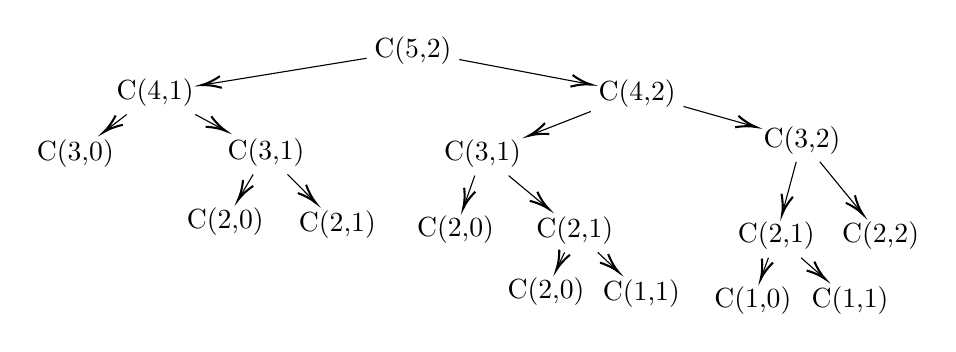
\begin{tikzpicture}[x=0.65pt,y=0.65pt,yscale=-1,xscale=1]
%uncomment if require: \path (0,300); %set diagram left start at 0, and has height of 300

\draw (319,26) node  [align=left] {C(5,2)};
\draw (443.67,49.67) node  [align=left] {C(4,2)};
\draw (535.33,75.67) node  [align=left] {C(3,2)};
\draw (175.67,49.33) node  [align=left] {C(4,1)};
\draw (357.67,83.33) node  [align=left] {C(3,1)};
\draw (237.33,82.67) node  [align=left] {C(3,1)};
\draw (131.33,83.33) node  [align=left] {C(3,0)};
\draw (342.67,125.67) node  [align=left] {C(2,0)};
\draw (277,122.67) node  [align=left] {C(2,1)};
\draw (214.67,121) node  [align=left] {C(2,0)};
\draw (521,129) node  [align=left] {C(2,1)};
\draw (409,126) node  [align=left] {C(2,1)};
\draw (446,161) node  [align=left] {C(1,1)};
\draw (393,160) node  [align=left] {C(2,0)};
\draw (579,129) node  [align=left] {C(2,2)};
\draw (562,165) node  [align=left] {C(1,1)};
\draw (508,165) node  [align=left] {C(1,0)};
\draw    (293.23,30.19) -- (203.41,44.82) ;
\draw [shift={(201.43,45.14)}, rotate = 350.75] [color={rgb, 255:red, 0; green, 0; blue, 0 }  ][line width=0.75]    (10.93,-3.29) .. controls (6.95,-1.4) and (3.31,-0.3) .. (0,0) .. controls (3.31,0.3) and (6.95,1.4) .. (10.93,3.29)   ;

\draw    (344.77,30.89) -- (415.94,44.4) ;
\draw [shift={(417.9,44.78)}, rotate = 190.75] [color={rgb, 255:red, 0; green, 0; blue, 0 }  ][line width=0.75]    (10.93,-3.29) .. controls (6.95,-1.4) and (3.31,-0.3) .. (0,0) .. controls (3.31,0.3) and (6.95,1.4) .. (10.93,3.29)   ;

\draw    (159.91,61.42) -- (148.68,70.03) ;
\draw [shift={(147.09,71.25)}, rotate = 322.51] [color={rgb, 255:red, 0; green, 0; blue, 0 }  ][line width=0.75]    (10.93,-3.29) .. controls (6.95,-1.4) and (3.31,-0.3) .. (0,0) .. controls (3.31,0.3) and (6.95,1.4) .. (10.93,3.29)   ;

\draw    (198.02,61.42) -- (213.22,69.63) ;
\draw [shift={(214.98,70.58)}, rotate = 208.39] [color={rgb, 255:red, 0; green, 0; blue, 0 }  ][line width=0.75]    (10.93,-3.29) .. controls (6.95,-1.4) and (3.31,-0.3) .. (0,0) .. controls (3.31,0.3) and (6.95,1.4) .. (10.93,3.29)   ;

\draw    (417.9,59.75) -- (385.3,72.52) ;
\draw [shift={(383.43,73.25)}, rotate = 338.62] [color={rgb, 255:red, 0; green, 0; blue, 0 }  ][line width=0.75]    (10.93,-3.29) .. controls (6.95,-1.4) and (3.31,-0.3) .. (0,0) .. controls (3.31,0.3) and (6.95,1.4) .. (10.93,3.29)   ;

\draw    (469.43,56.98) -- (507.64,67.81) ;
\draw [shift={(509.57,68.36)}, rotate = 195.84] [color={rgb, 255:red, 0; green, 0; blue, 0 }  ][line width=0.75]    (10.93,-3.29) .. controls (6.95,-1.4) and (3.31,-0.3) .. (0,0) .. controls (3.31,0.3) and (6.95,1.4) .. (10.93,3.29)   ;

\draw    (230.19,94.75) -- (222.83,107.2) ;
\draw [shift={(221.81,108.92)}, rotate = 300.6] [color={rgb, 255:red, 0; green, 0; blue, 0 }  ][line width=0.75]    (10.93,-3.29) .. controls (6.95,-1.4) and (3.31,-0.3) .. (0,0) .. controls (3.31,0.3) and (6.95,1.4) .. (10.93,3.29)   ;

\draw    (249.32,94.75) -- (263.61,109.16) ;
\draw [shift={(265.02,110.58)}, rotate = 225.24] [color={rgb, 255:red, 0; green, 0; blue, 0 }  ][line width=0.75]    (10.93,-3.29) .. controls (6.95,-1.4) and (3.31,-0.3) .. (0,0) .. controls (3.31,0.3) and (6.95,1.4) .. (10.93,3.29)   ;

\draw    (353.39,95.42) -- (347.62,111.7) ;
\draw [shift={(346.95,113.58)}, rotate = 289.51] [color={rgb, 255:red, 0; green, 0; blue, 0 }  ][line width=0.75]    (10.93,-3.29) .. controls (6.95,-1.4) and (3.31,-0.3) .. (0,0) .. controls (3.31,0.3) and (6.95,1.4) .. (10.93,3.29)   ;

\draw    (372.2,95.42) -- (392.92,112.64) ;
\draw [shift={(394.46,113.92)}, rotate = 219.73] [color={rgb, 255:red, 0; green, 0; blue, 0 }  ][line width=0.75]    (10.93,-3.29) .. controls (6.95,-1.4) and (3.31,-0.3) .. (0,0) .. controls (3.31,0.3) and (6.95,1.4) .. (10.93,3.29)   ;

\draw    (403.31,138.08) -- (399.54,146.11) ;
\draw [shift={(398.69,147.92)}, rotate = 295.2] [color={rgb, 255:red, 0; green, 0; blue, 0 }  ][line width=0.75]    (10.93,-3.29) .. controls (6.95,-1.4) and (3.31,-0.3) .. (0,0) .. controls (3.31,0.3) and (6.95,1.4) .. (10.93,3.29)   ;

\draw    (421.77,138.08) -- (431.77,147.54) ;
\draw [shift={(433.23,148.92)}, rotate = 223.41] [color={rgb, 255:red, 0; green, 0; blue, 0 }  ][line width=0.75]    (10.93,-3.29) .. controls (6.95,-1.4) and (3.31,-0.3) .. (0,0) .. controls (3.31,0.3) and (6.95,1.4) .. (10.93,3.29)   ;

\draw    (532.09,87.75) -- (524.77,114.99) ;
\draw [shift={(524.25,116.92)}, rotate = 285.04] [color={rgb, 255:red, 0; green, 0; blue, 0 }  ][line width=0.75]    (10.93,-3.29) .. controls (6.95,-1.4) and (3.31,-0.3) .. (0,0) .. controls (3.31,0.3) and (6.95,1.4) .. (10.93,3.29)   ;

\draw    (545.23,87.75) -- (567.84,115.37) ;
\draw [shift={(569.11,116.92)}, rotate = 230.69] [color={rgb, 255:red, 0; green, 0; blue, 0 }  ][line width=0.75]    (10.93,-3.29) .. controls (6.95,-1.4) and (3.31,-0.3) .. (0,0) .. controls (3.31,0.3) and (6.95,1.4) .. (10.93,3.29)   ;

\draw    (516.64,141.08) -- (513.04,151.04) ;
\draw [shift={(512.36,152.92)}, rotate = 289.86] [color={rgb, 255:red, 0; green, 0; blue, 0 }  ][line width=0.75]    (10.93,-3.29) .. controls (6.95,-1.4) and (3.31,-0.3) .. (0,0) .. controls (3.31,0.3) and (6.95,1.4) .. (10.93,3.29)   ;

\draw    (534.76,141.08) -- (546.74,151.6) ;
\draw [shift={(548.24,152.92)}, rotate = 221.28] [color={rgb, 255:red, 0; green, 0; blue, 0 }  ][line width=0.75]    (10.93,-3.29) .. controls (6.95,-1.4) and (3.31,-0.3) .. (0,0) .. controls (3.31,0.3) and (6.95,1.4) .. (10.93,3.29)   ;
\end{tikzpicture}

\end{frame}

\begin{frame}{Algorithm for C(n,r)}
    \SetKwProg{Fn}{Function}{}{}
    \begin{algorithm}[H]
    \SetAlgoLined
        \Fn{nCr (n,r)}{
            \If{r==1}{
                return n\;
            }
            
            \If{r=n or r=0}{
                return 1\;
            }
            
            \If{dp[n][r] already calculated}{
                return dp[n][r];   //use of memoization\\
            }
            
            dp[n][r]=nCr(n-1,r)+nCr(n-1,r-1);\\
            return dp[n][r]; 
        }
    \end{algorithm}
\end{frame}

\begin{frame}{}
    
    \centering
    \tikzset{every picture/.style={line width=0.75pt}} %set default line width to 0.75pt        
    
    
\begin{tikzpicture}[x=0.75pt,y=0.75pt,yscale=-1,xscale=1]
    %uncomment if require: \path (0,300); %set diagram left start at 0, and has height of 300
    
    \draw  [color={rgb, 255:red, 74; green, 144; blue, 226 }  ,draw opacity=1 ][line width=2.25]   (312, 108.08) circle [x radius= 35, y radius= 29.92]  ;
    \draw  [color={rgb, 255:red, 74; green, 144; blue, 226 }  ,draw opacity=1 ][line width=6]   (295.65, 97.02) circle [x radius= 0.02, y radius= 0.02]  ;
    \draw  [color={rgb, 255:red, 74; green, 144; blue, 226 }  ,draw opacity=1 ][line width=6]   (325.65, 97.02) circle [x radius= 0.02, y radius= 0.02]  ;
    \draw  [color={rgb, 255:red, 74; green, 144; blue, 226 }  ,draw opacity=1 ] (294.63,116) .. controls (305.75,132.72) and (316.88,132.72) .. (328,116) ;
    
    \draw (322,182) node  [align=left] {{\Large \textcolor[rgb]{0.29,0.56,0.89}{Thanks !! Any Questions??}}};
    
    
    \end{tikzpicture}

\end{frame}


\end{document}
